\chapter{The \lhcb detector}
\label{sec:Detector}
The Large Hadron Collider (LHC) of the European Organization for Nuclear Research CERN in Geneva, Switzerland is currently the world's most powerful particle accelerator.
Having a circumference of 26.7 \km it is designed to either collide protons with a centre-of-mass energy of $\sqs=14\tev$ or heavy ions with 2.8 \tev per nucleon \cite{LHC}.
The beams can be brought to collision at four interaction points.
At these points different experiments are placed.
Whereas \atlas and \cms are built as multi-purpose detectors \cite{ATLAS, CMS} and \alice studies heavy-ion collisions \cite{ALICE}, \lhcb is dedicated to search indirectly for evidence of physics beyond the Standard Model by the study of hadrons containing either a heavy \bquark- or \cquark-quark.

Those \B- and \D-hadrons are mainly produced by gluon-gluon fusion at \lhc energies with subsequent hadronisation.
These gluons in general carry different momenta leading to a boost of the hadron along the beam-pipe.
This is why the \lhcb detector is built as a single-arm forward spectrometer.
Its layout can be seen in figure \ref{fig:detector}.
\begin{figure}[hptb]
    \centering
	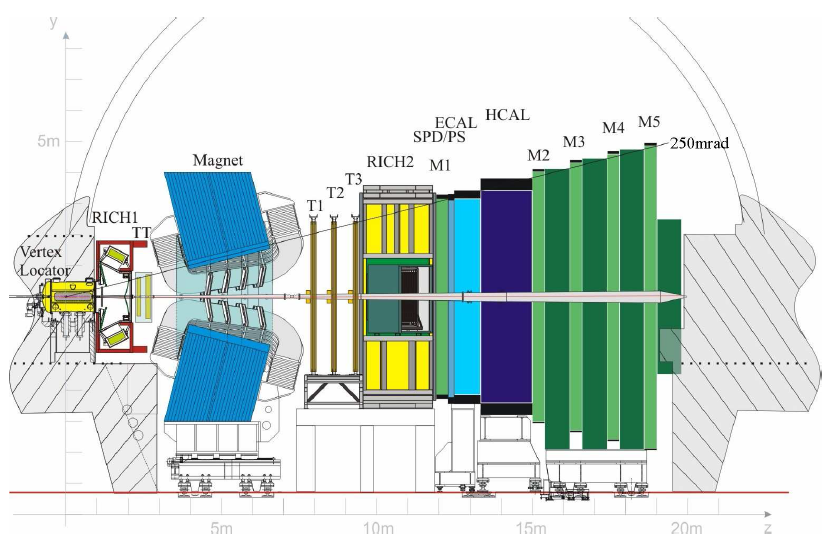
\includegraphics[width=\textwidth]{lhcb-detector}	
	\caption{The \lhcb detector.}
	\label{fig:detector}
\end{figure}
It has a forward angular coverage from approximately 10\mrad to 300\mrad in the bending respectively to 250\mrad in the non-bending plane.
A right-handed coordinate system is adopted with the $z$ axis along the beam-pipe and the $y$ axis pointing upwards along the vertical.
With this choice approximately 25\% of all \bquark\bquarkbar pairs are produced in the acceptance of the \lhcb detector \cite{bb_Production} though it covers only 4\% of the solid angle as shown in Figure \ref{fig:bb_Production}.
\begin{figure}[hptb]
    \centering
	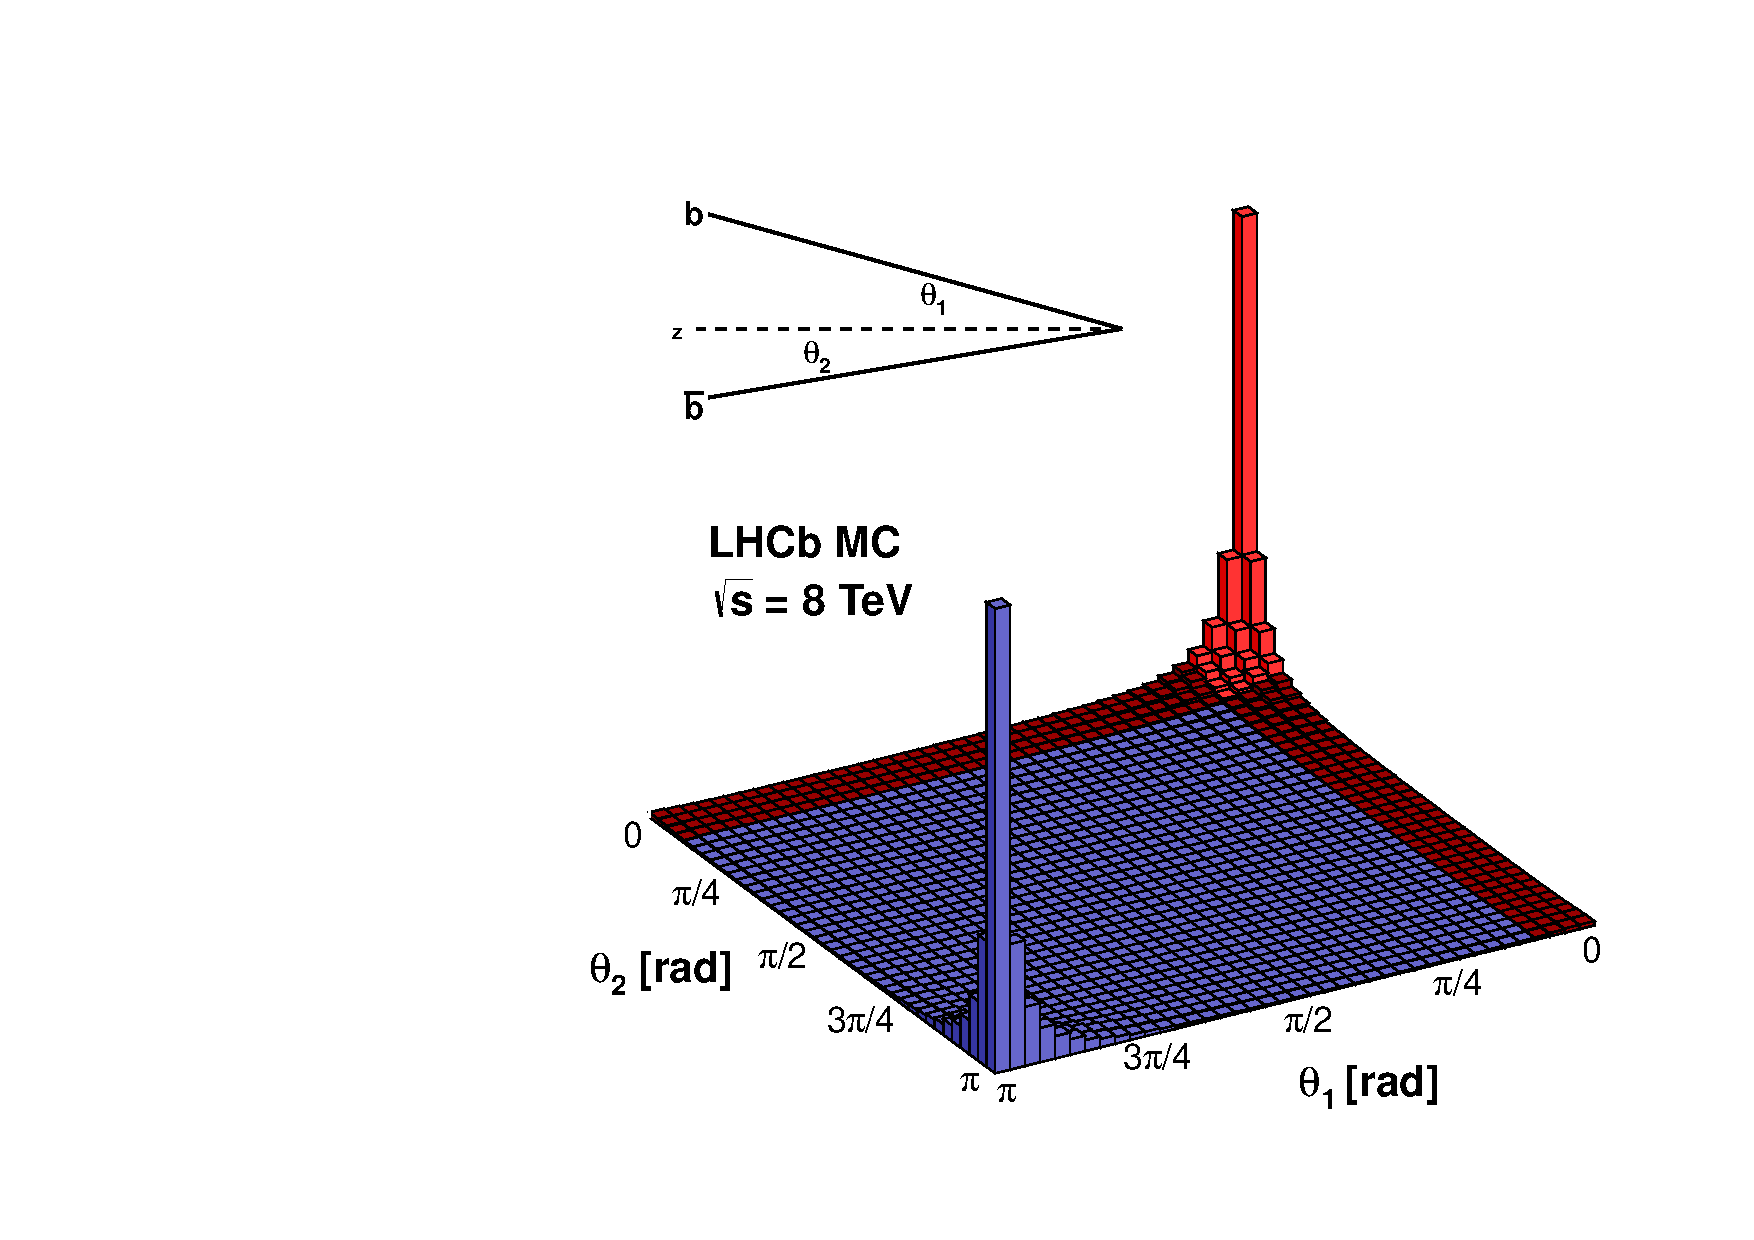
\includegraphics[width=0.5\textwidth]{bb_production}	
	\label{fig:bb_Production}
    \caption{Simulation of the \bquark\bquarkbar production in \proton\proton collisions at $\protect\sqs = 8 \protect\tev$.
             The angular acceptance of the \lhcb detector is coloured in red. Figure taken from.}
\end{figure}
The \lhcb detector consists of multiple subdetectors and sensors.
They can be roughly separated into two groups by their dedicated purpose.
They are in priciple either used for the reconstruction of particle tracks or to identify the particles.
Both groups will be explained in the following.

% ===========================
% SECTION: Tracking detectors
% ===========================
\section{Tracking detectors}
Tracking describes the whole procedure to reconstruct the trajectories of (charged) particles produced in the proton-proton collision. 
Together with the dipole magnet, the particles' charges and momenta can be determined as well by the deflection of the track.
The magnet provides a magnetic field of 4\unit{Tm} integrated over a length of 10\m.
Its main component, the magnetic field in $y$ direction, is shown in Figure \ref{fig:MagneticField_Tracks}.
For the particle tracking, a system of several subdetectors is aligned up- and downstream the dipole magnet, namely the Vertex locator (VELO), the Trigger Tracker (TT) and the Trigger stations (T1-T3) built-up by the Inner Tracker (IT) and the Outer Tracker (OT).

\subsection{Vertex Locator (VELO)}
The VErtex LOcator (VELO) is placed directly around the primary interaction point. 
Its task is to precisely measure the track coordinates of charged particles and separate the proton-proton interaction point from other vertices, namely either other primary vertices (so called pile-up events) or secondary vertices. 
The latter ones are typically for \bquark- or \cquark-hadron decays \cite{VELO_TDR} and a good separation and resolution of these vertices is crucial for the \lhcb physics programme.
As an example serves the measurement of particles' decay length and time for the determination of the rapid $\Bs-\Bsb$ oscillation frequency \cite{BsBsbar_frequency}.

The VELO is built up by silicon modules due to the high particle flux and thus high radiation in the interaction region. 
It is placed only 7\mm apart from the beam. 
This is closer than the required aperture of the \lhcb beam pipe at injection. 
Thus, the VELO sensors are made of silicon microstrips shaped as slightly overlapping half-discs. 
The two halfs can be moved in $x$- and $y$-direction to avoid radiation damages unless the beam is stable.

Each module provides a measurement of the $r$- and $\phi$-coordinates.
The sensores for these measurements are correspondingly called $R$- and $\Phi$-sensor, which can be seen in figure \ref{fig:VELO_RandPhiSensor}.
An overview over the VELO system with its modules is shown in figure \ref{fig:VELO_Overview}. 
Around the nominal interaction region, the modules are placed closer to each other. 
Upstream there are two $R$ sensors dedicated to veto pile-up events. 
Figure \ref{fig:VELO_Overview} furthermore shows the VELO in closed and opened position.
\begin{figure}[hptb]
    \centering
	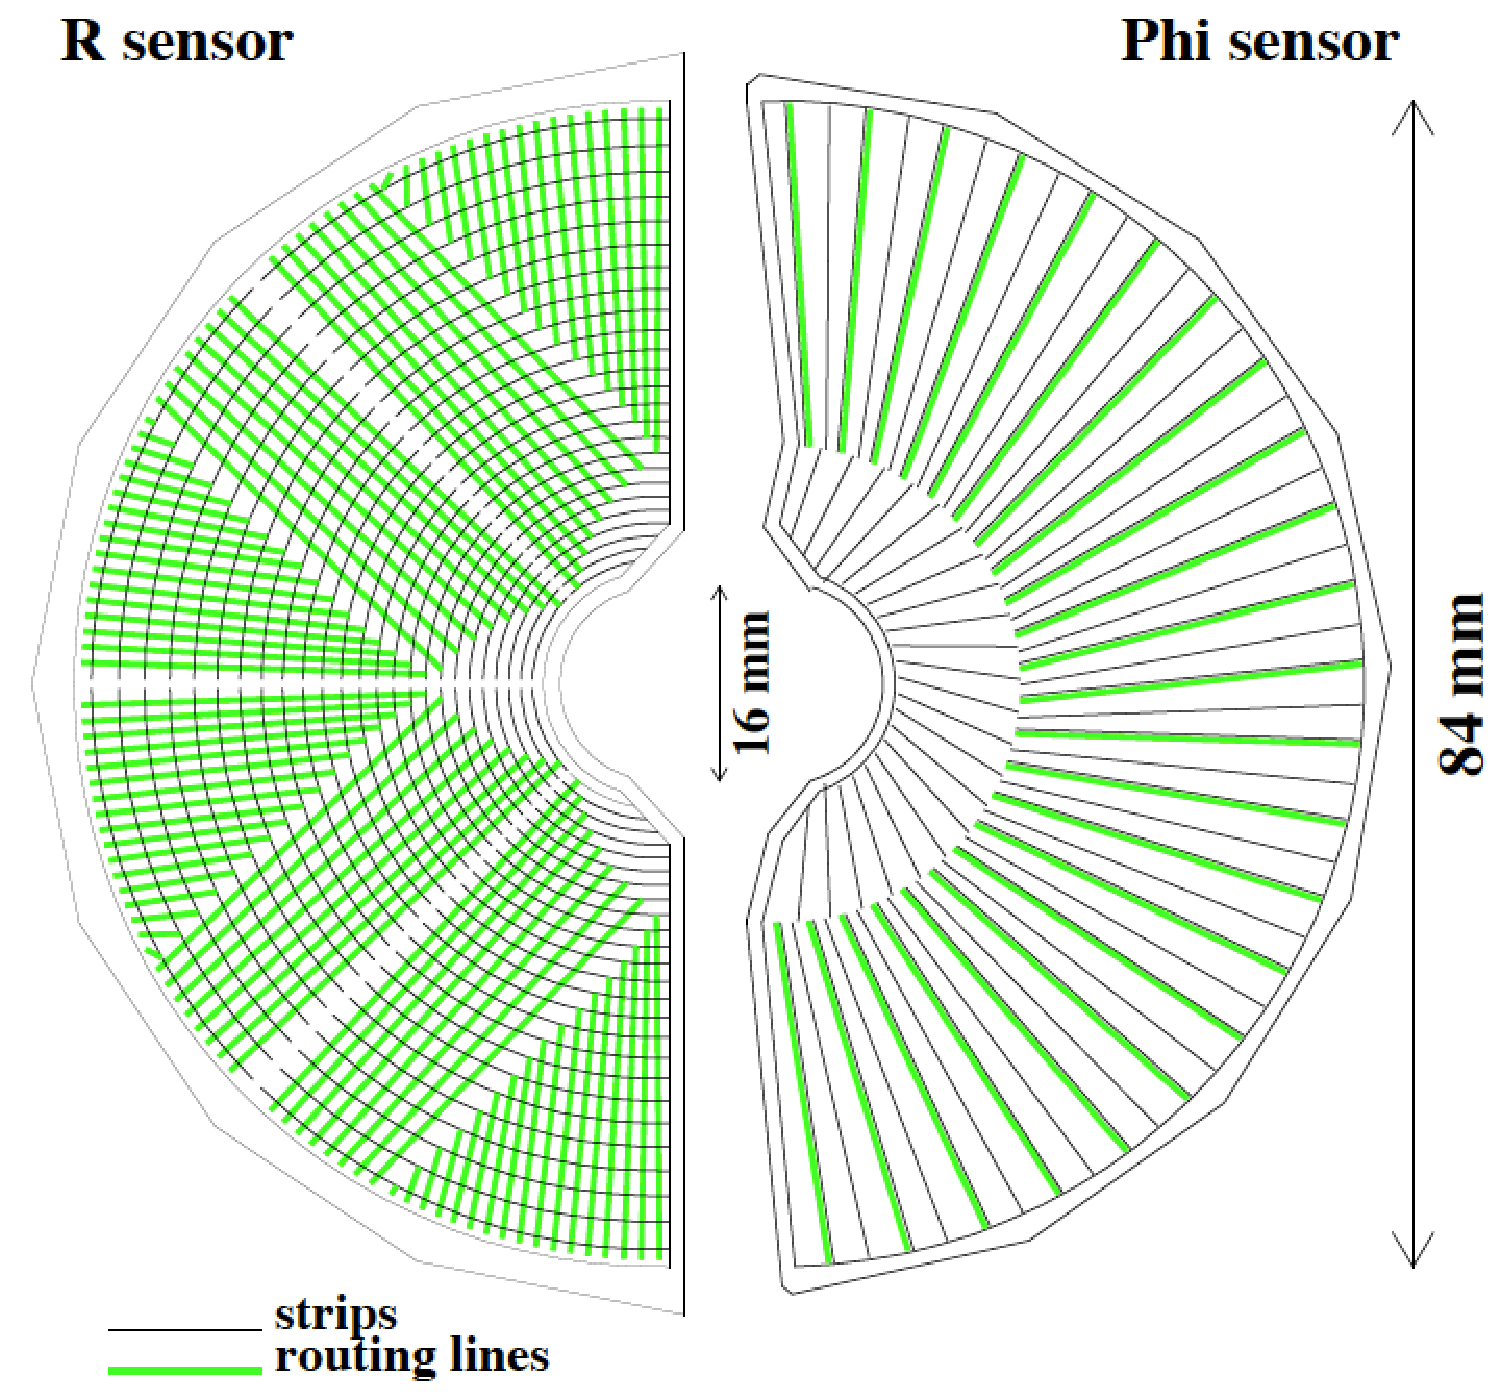
\includegraphics[width=0.5\textwidth]{VELO_randphisensors}	
	\caption{Schematic representation of an $R$ and a $\Phi$ sensor. The $R$ sensor strips are arranged into four approximately 45\degrees segments and have routing lines perpendicular to the strips. The $\Phi$ sensor has two zones with inner and outer strips. The routing lines of the inner strips
    are orientated parallel to the outer strips. Figure and caption taken from \cite{VELO_Performance}.}
	\label{fig:VELO_RandPhiSensor}
\end{figure}
\begin{figure}[hptb]
    \centering
	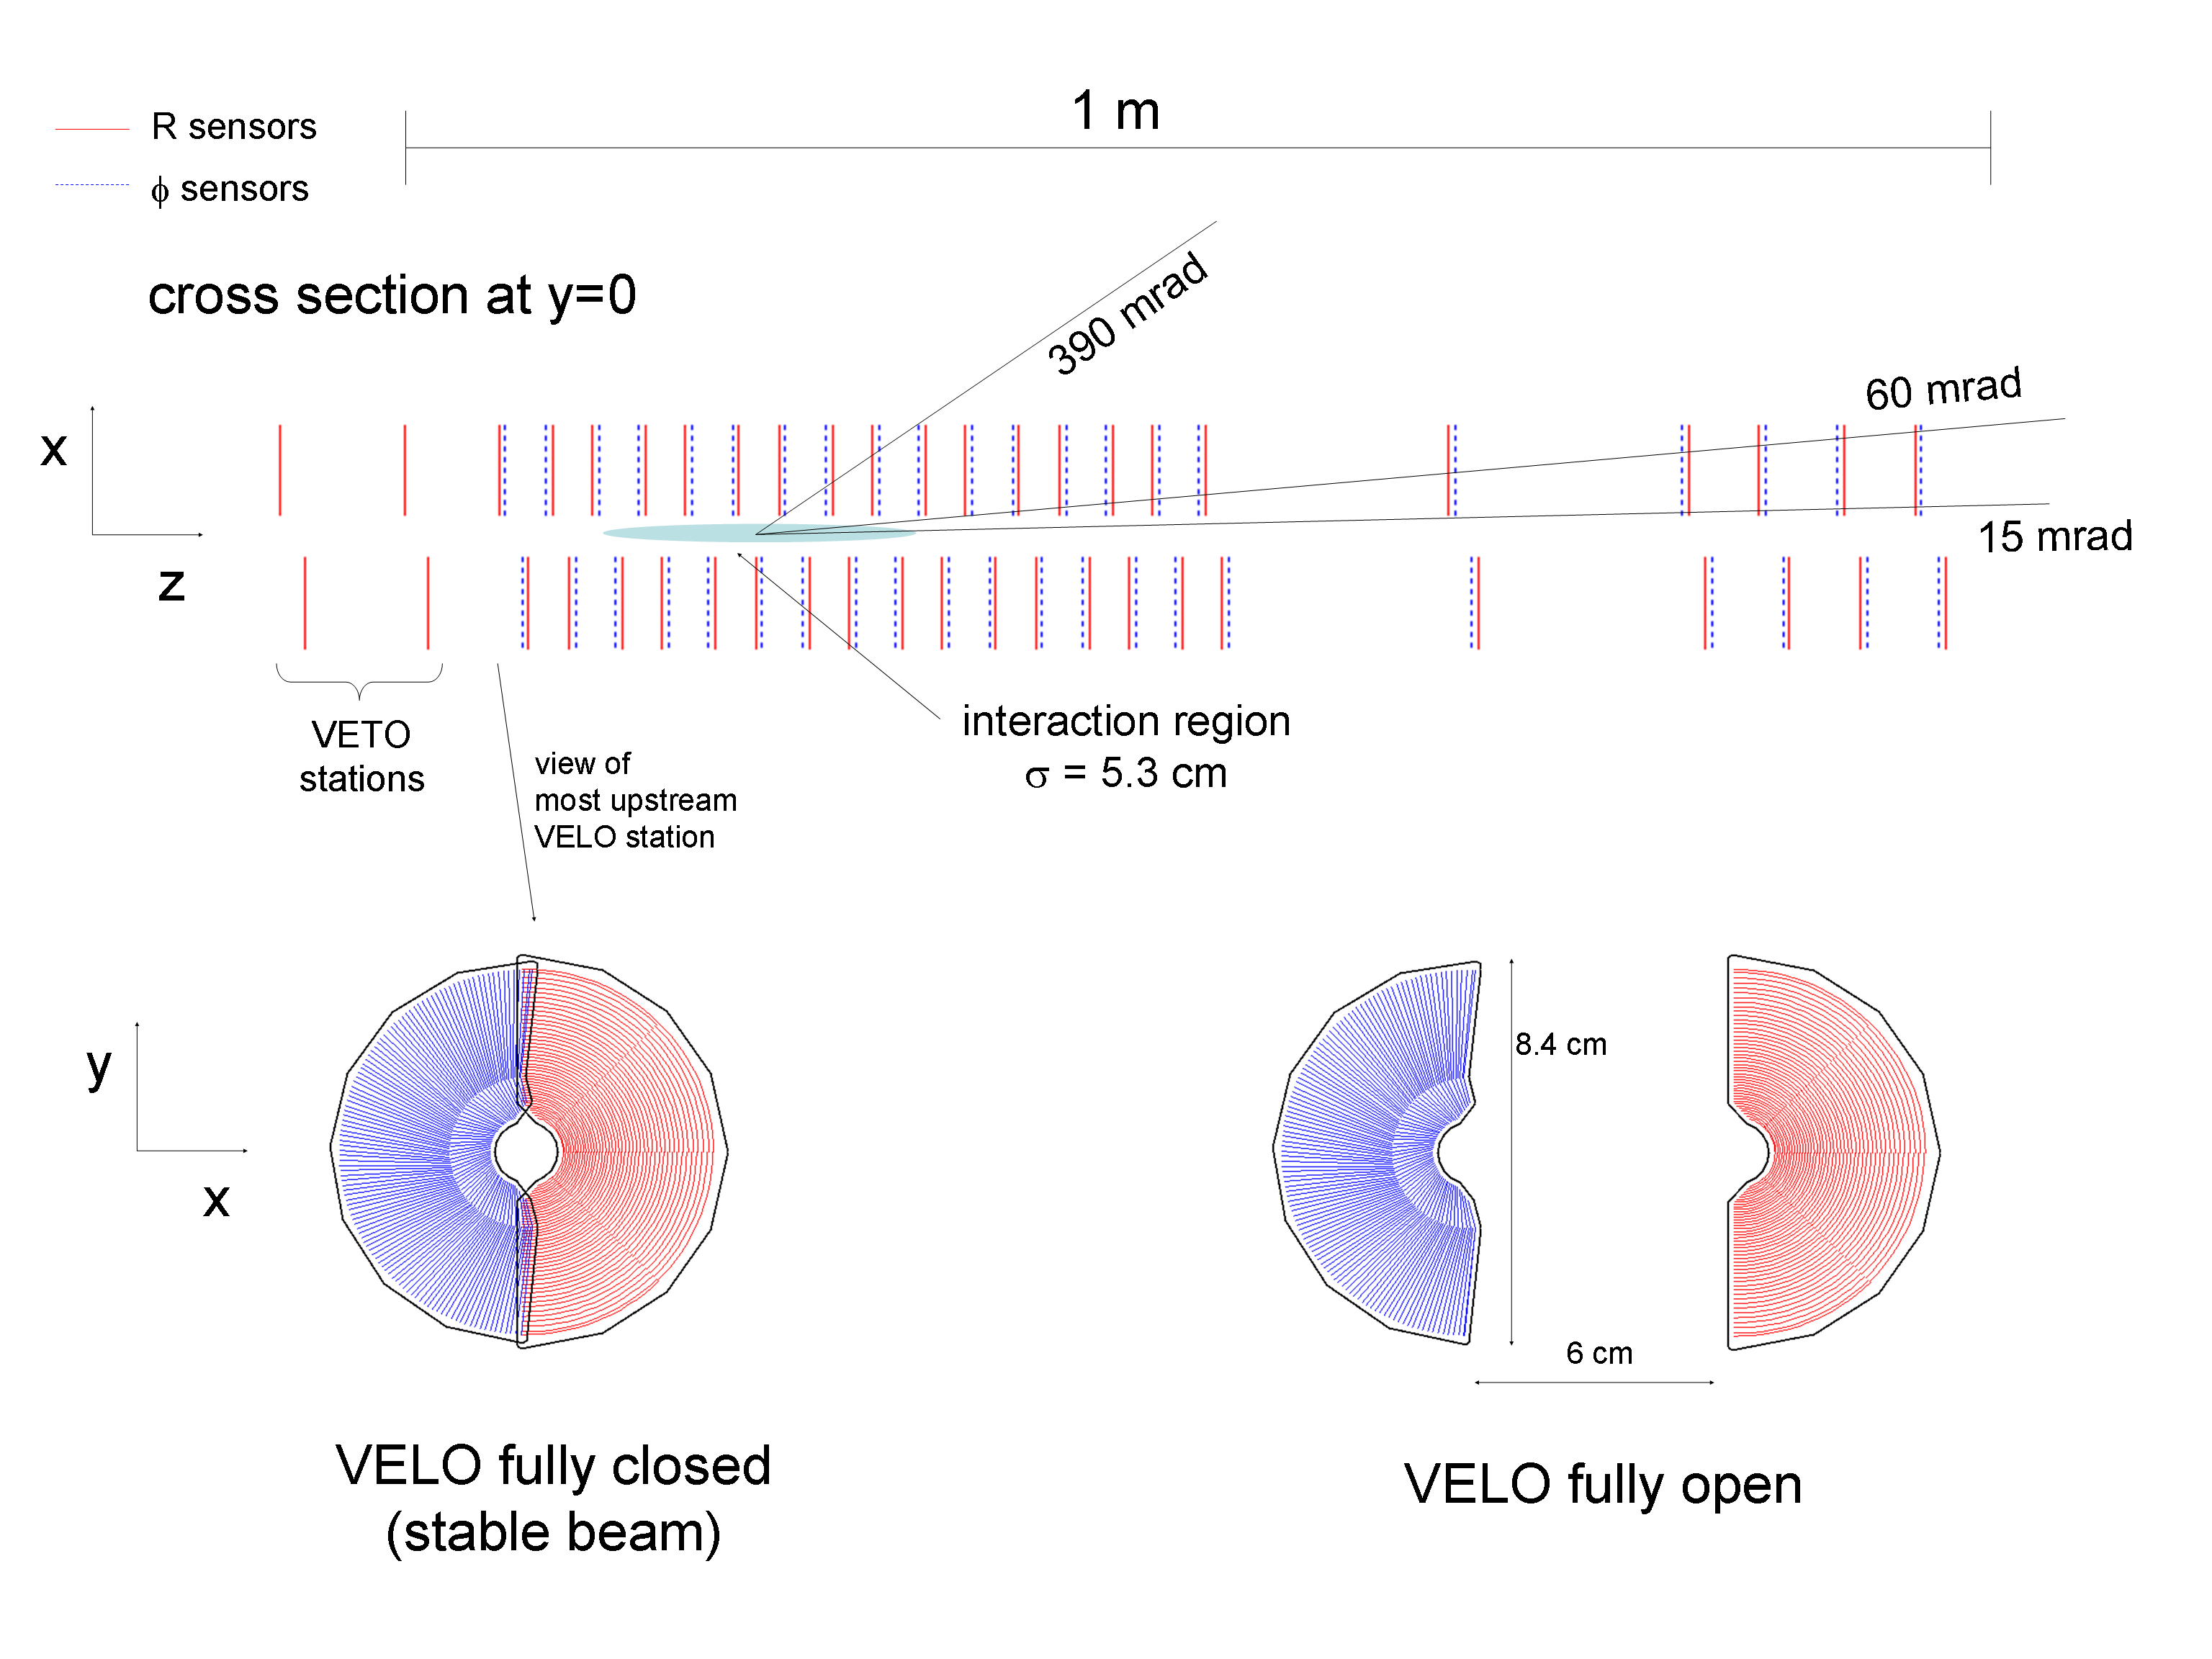
\includegraphics[width=0.8\textwidth]{VELO_Overview}	
	\caption{Cross section in the $(x,z)$ plane of the VELO silicon sensors, at $y=0$, with the detector in the fully closed position. 
             The front face of the first modules is also illustrated in both the closed and open positions. 
             The two pile-up veto stations are located upstream of the VELO sensors.
             Figure and caption taken from \cite{detector}.}
	\label{fig:VELO_Overview}
\end{figure}
With this setup the VELO reaches a track finding efficiency above 98\%. 
Its resolution on vertices is 13\mum in the transverse plane and 71\mum along the beam axis for vertices with 25 tracks. 
The resolution on the impact parameter is smaller than 35\mum for particles with a transverse momentum larger than 1\gev \cite{detector, VELO_TDR, VELO_Performance}.

\subsection{Silicon Tracker (ST)}
The Silicon Tracker (ST) uses silicon microstrip detectors with a strip pitch of about 200\mum.
It comprises two detectors: the Tracker Truciensis (TT) and the Inner Tracker (IT).
The Tracker Turicencis or formerly the Trigger Tracker is located in front of the entrance of the \lhcb magnet. 
It is used for sevaral tasks:
\begin{itemize}
    \item deliver transverse momentum information for Level-1 trigger,
    \item reconstruct trajectories of long-lived neutral particles decaying outside the VELO
    \item reconstruct low-momenta particles bent out by the magnet before reaching the station T1-T3.
\end{itemize}
The TT consists of one station made of four planes along the beam axis. 
The first and the fourth layer have vertical readout strips ($x$-layer), while the second and third are rotated by an angle $\pm 5\degrees$ to get a high resolution in the bending plane and additional information in $y$-direction.
Between the $u$ and $v$ layer there is a gap of around 30\cm. 
Figure \ref{fig:TT_layers} shows schematically the layout of the TT.
\begin{figure}[hptb]
    \centering
	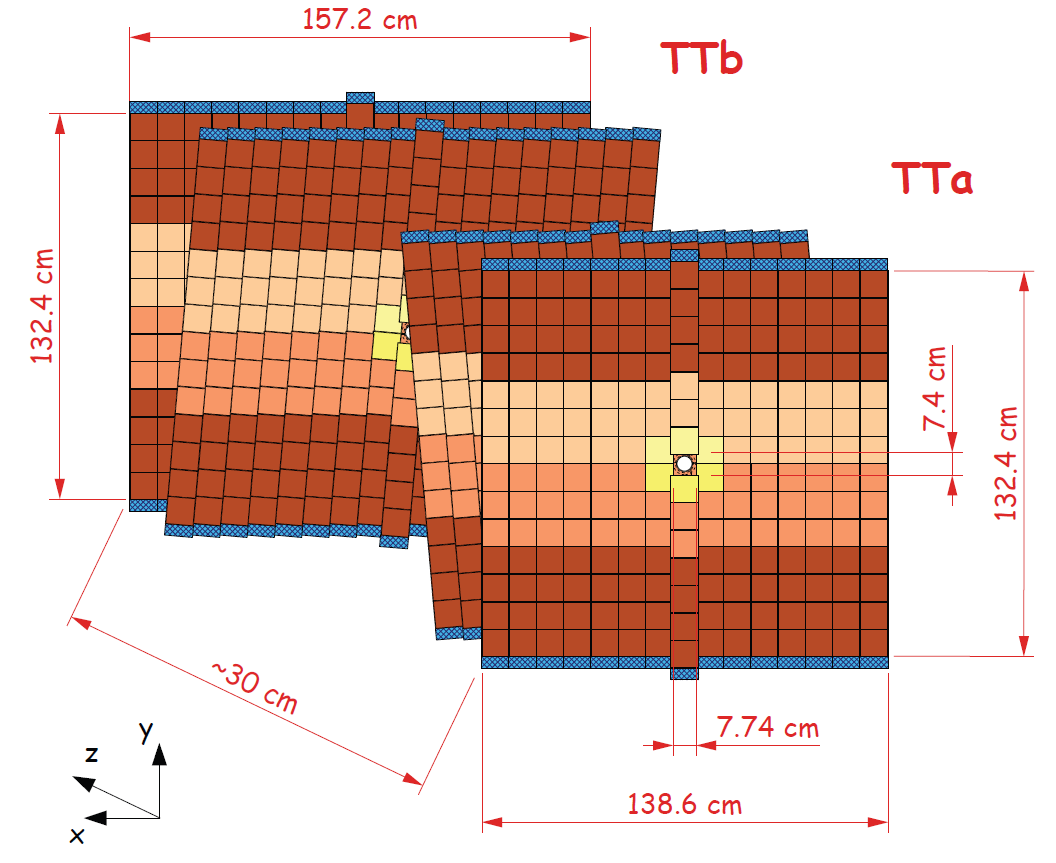
\includegraphics[width=0.8\textwidth]{TT_layers}	
	\caption{Layout of the Tracker Turicensis (TT). 
             Figure taken from \cite{ST_Performance}.}
	\label{fig:TT_layers}
\end{figure}
The Inner Tracker uses the same technology as the TT as already mentioned. 
It builds the inner part of the three tracking stations T1-T3 (see Figure \ref{fig:detector}), which are located downstream the magnet.
Each station consists of four boxes as shown in figure \ref{fig:IT_layer}.
In each box there are again 4 layers, two vertical and two stereo, analogously to the TT. 
Though the IT only covers 1.3\% of the geometrical acceptance, 20\% of the track are passing it \cite{detector, ST_Performance}.
\begin{figure}[hptb]
    \centering
	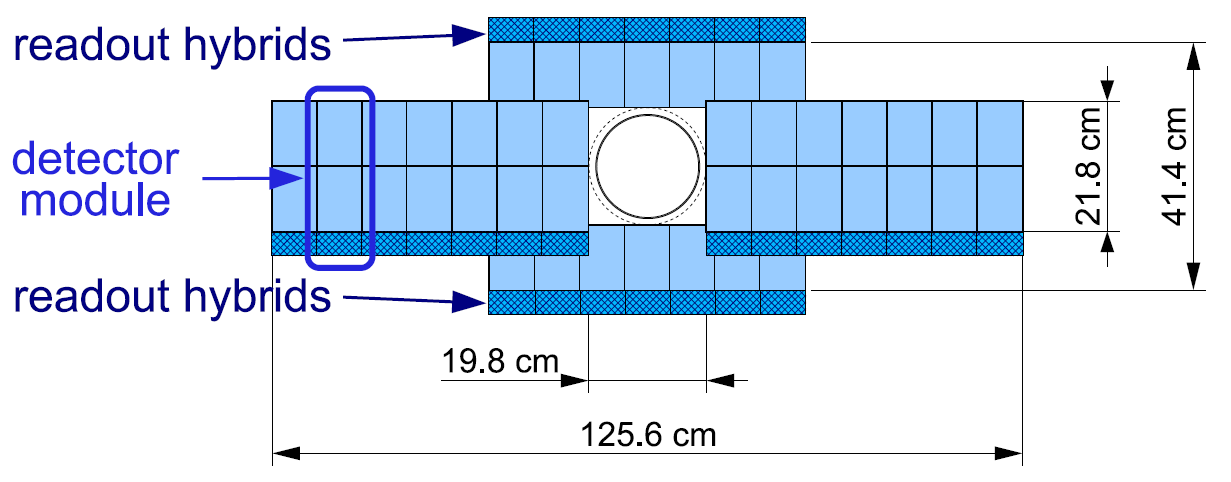
\includegraphics[width=0.8\textwidth]{IT_layer}	
	\caption{Layout of a $x$ detection layer in the second Inner Tracker (IT) station. 
             Figure taken from \cite{detector}.}
	\label{fig:IT_layer}
\end{figure}

\subsection{Outer Tracker (OT)}
The Outer Tracker builds the outer part of the Tracking stations T1-T3 downstream the magnet.
It is a gaseous straw tube detector covering an area of approximately $5 \times 6 \ma$ with 12 double layers of straw tubes.
The straw tubes are filled with a gas mixture of argon (70\%), carbon dioxide (28.5\%) and oxygen (1.5\%).
This guarantees a drift time of less than 50\ns enabling to distinguish consecutive proton bunch collisions.
Again the three stations consist of 4 layers each in $x-u-v-x$ geometry.
The spatial resolution is 200\mum along the $x$ axis.
On the one hand this is worse than the spatial resolution of the IT with 50\mum, but on the other hand the angular coverage is much higher \cite{OT_Performance}.

\subsection{Track classification}
For the reconstruction of tracks the registered hits of the VELO, TT, IT and OT are combined to form particle trajectories.
Depending on the trajectories one defines different classes of trajectories, which are also sketched in Figure \ref{fig:MagneticField_Tracks}:
\begin{itemize}
    \item \textsc{Long tracks} traverse the full tracking system from the VELO to the T stations.
          Note: In this analysis only long tracks are used.
    \item If particles traverse the VELO and TT stations only, their tracks are called \textsc{upstream tracks}.
    \item Particles decaying outside the VELO acceptance and leaving hits only in the TT and T stations are called \textsc{downstream tracks}.
    \item \textsc{VELO tracks} are measured in the VELO only.
    \item \textsc{T tracks} only traverse the T stations.
\end{itemize}
\begin{figure}[hptb]
    \centering
	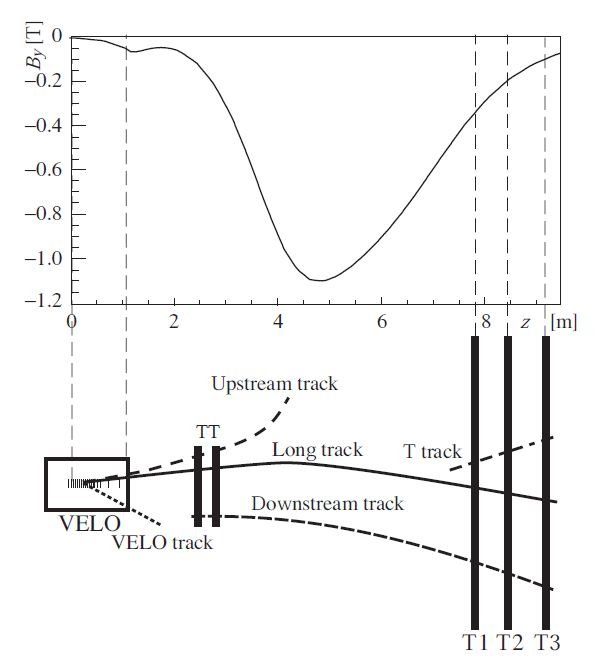
\includegraphics[width=0.5\textwidth]{MagneticField_Tracks}	
	\caption{A schematic illustration of the various track types: long, upstream, downstream, VELO and T tracks.
             For reference the main $B$-field component $B_y$ is plotted above as function of the $z$ coordinate.
             Figure and caption taken from \cite{LHCb_Reoptimization}.}
	\label{fig:IT_layer}
\end{figure}

% ================================
% SECTION: Particle identification
% ================================
\section{Particle identification}
The reconstruction of \bquark- and \cquark- hadrons require the identification of the particles associated to the reconstructed tracks.
Several facilities for that purpose are available at the \lhcb detector, that are described in the following.

\subsection{Ring Imaging Cherenkov Detector (RICH)}
The RICH detectors at \lhcb are dedicated to distinguish charged hadrons espeacially pions, kaons and hadrons.
They make use of the Cherenkov radiation.
If charged particles fly through a dielectric medium with a velocity $\beta = v/c$ that is faster as the speed of light in that medium, they emit photons in a cone around their flight path.
The opening angle $\theta_C$ of that light cone is given by
\begin{align}
    \cos \theta_C = \frac{1}{\beta n},
\end{align}
where $n$ denotes the refractive index of the medium \cite{Jackson_ED}.
\lhcb's RICH detectors measure the opening angle of the Cherenkov cone and use it to determine the velocity.
Together with the measured momenta from tracking it is possible to calculate the mass of the particle and thus to identify it.
The \lhcb detector consists of two RICH detectors.
RICH1 is located upstream the magnet before particles might bent out of the \lhcb detector acceptance by the magnet..
It contains aerogel and \cfourften gas and is dedicated to measure low-momenta particles between 1 \gev and 60 \gev.
However, RICH2 is placed downstream the magnet, filled with \cffour gas and covers the high-momentum range from 15 \gev to 100 \gev \cite{detector, RICH_Performance}.

\subsection{Calorimeter system}
The main purpose of the calorimeter system is to measure the energy of the particles.
Furthermore, it provides the identification of electrons, photons and hadrons and delivers trigger signals from photons, electrons and hadrons with high transverse momentum.
It contains several subsystems which are all located downstream the magnet.
The first part of the calorimeter system is the scintillating pad detector (SPD).
It is used to select charged particles and above all to distinguish between electrons and photons in the subsequent calorimeter parts.
After a 2.5 radiation lengths lead wall it is followed by the preshower detector (PS) identifying electromagnetic particles.
To measure the energy of electromagnetic particles, the electromagnetic calorimeter (ECAL) is placed behind the PS.
It uses the so called shashlik-technology, i.e. it employs an alternating structure of scintillating tiles and lead plates.
The last part of the calorimeter system is the hadronic calorimeter (HCAL).
It is a sampling device made of iron as absorber and scintillating tiles as active material and measures the energy of hadrons.

Basically, all calorimeters obey the same principle:
Scintillation light is transmitted to a Photo-Multiplier (PMT) by wavelength-shifting fibres.
Multianode photomultiplier tubes (MAPMT) read out the single fibres of the SPD / PS cells.
Fibre bunches in the ECAL and HCAL modules require individual phototubes \cite{detector, PS_SPD, Calorimeter_Running, ECAL, HCAL}.

\subsection{Muon chambers}
Muons as long-lived and minimum ionising particles can penetrate the whole detector.
That is why the muon chambers for the identification of muons are the last part of the detector.
There are five muon stations, one (M1) before the calorimeter system and four (M2-M5) behind.
To ensure that only muons penetrate the whole system the latter ones are interleaved with 80\cm thick iron absorbers.
Besides for the inner part of M1, the muon chambers mainly consist of multi-wire proportional chambers (MWPC) providing a fast readout.
In the inner part of M1 a gas electron multiplier is used due to the high particle flux \cite{detector, Muon_Performance}.

% ===========================
% SECTION: Trigger
% ===========================
\section{Trigger}
The LHC is designed to cross proton bunches every 25\ns.
This is equivalent to a beam crossing rate of 40\mhz.
However, it is not possible to record data at this rate.
Thus, the task of the \lhcb trigger system is to reduce the rate to a recordable level.
It has to decide quickly if an event is of interest for the \lhcb physics programme.
For this purpose, the trigger system is made up of three stages.

The first stage, the Level-0 (L0) trigger, is completely based on hardware.
It reduces the beam crossing rate of 40\mhz down to 1\mhz.
Due to the high rate, a full event reconstruction is not possible at this stage.
Thus, the L0 trigger only tries to reconstruct
\begin{itemize}
    \item the highest transverse energy \et hadron, electron and photon clusters in the calorimeters,
    \item the two highest transverse momentum muons in the muon chambers,
\end{itemize}
because \B mesons often produce large transverse momentum respectively energy particles due to their large mass \cite{detector}.
Furthermore the pile-up system in the VELO is used to estimate the number of primary \proton\proton interactions per bunch-crossing.

The L0 trigger is followed by the software based high-level trigger HLT.
The HLT itself is subdivided into the HLT1 and the HLT2.
Events passing the L0 trigger enter the HLT1 with a rate of about 1\mhz.
Due to limited computing power only a partial event reconstruction using particles in the VELO and T stations is possible.
The decision if an event passes the trigger or not is mainly based on the track quality.
This reduces the event rate to about 40\khz and enables HLT2 to fully reconstruct the event.
The information of all \lhcb subsystems are available at this stage which allows a more advanced selection.
The event rate is reduced to 5\khz by HLT2, which is low enough to store the data on disk \cite{detector, Trigger, Trigger_Performance_2011}.

